% Options for packages loaded elsewhere
\PassOptionsToPackage{unicode}{hyperref}
\PassOptionsToPackage{hyphens}{url}
%
\documentclass[
]{book}
\title{Comandos básicos do R: Guia de bolso}
\author{Lucas C. Germano}
\date{2022-05-14}

\usepackage{amsmath,amssymb}
\usepackage{lmodern}
\usepackage{iftex}
\ifPDFTeX
  \usepackage[T1]{fontenc}
  \usepackage[utf8]{inputenc}
  \usepackage{textcomp} % provide euro and other symbols
\else % if luatex or xetex
  \usepackage{unicode-math}
  \defaultfontfeatures{Scale=MatchLowercase}
  \defaultfontfeatures[\rmfamily]{Ligatures=TeX,Scale=1}
\fi
% Use upquote if available, for straight quotes in verbatim environments
\IfFileExists{upquote.sty}{\usepackage{upquote}}{}
\IfFileExists{microtype.sty}{% use microtype if available
  \usepackage[]{microtype}
  \UseMicrotypeSet[protrusion]{basicmath} % disable protrusion for tt fonts
}{}
\makeatletter
\@ifundefined{KOMAClassName}{% if non-KOMA class
  \IfFileExists{parskip.sty}{%
    \usepackage{parskip}
  }{% else
    \setlength{\parindent}{0pt}
    \setlength{\parskip}{6pt plus 2pt minus 1pt}}
}{% if KOMA class
  \KOMAoptions{parskip=half}}
\makeatother
\usepackage{xcolor}
\IfFileExists{xurl.sty}{\usepackage{xurl}}{} % add URL line breaks if available
\IfFileExists{bookmark.sty}{\usepackage{bookmark}}{\usepackage{hyperref}}
\hypersetup{
  pdftitle={Comandos básicos do R: Guia de bolso},
  pdfauthor={Lucas C. Germano},
  hidelinks,
  pdfcreator={LaTeX via pandoc}}
\urlstyle{same} % disable monospaced font for URLs
\usepackage{color}
\usepackage{fancyvrb}
\newcommand{\VerbBar}{|}
\newcommand{\VERB}{\Verb[commandchars=\\\{\}]}
\DefineVerbatimEnvironment{Highlighting}{Verbatim}{commandchars=\\\{\}}
% Add ',fontsize=\small' for more characters per line
\usepackage{framed}
\definecolor{shadecolor}{RGB}{248,248,248}
\newenvironment{Shaded}{\begin{snugshade}}{\end{snugshade}}
\newcommand{\AlertTok}[1]{\textcolor[rgb]{0.94,0.16,0.16}{#1}}
\newcommand{\AnnotationTok}[1]{\textcolor[rgb]{0.56,0.35,0.01}{\textbf{\textit{#1}}}}
\newcommand{\AttributeTok}[1]{\textcolor[rgb]{0.77,0.63,0.00}{#1}}
\newcommand{\BaseNTok}[1]{\textcolor[rgb]{0.00,0.00,0.81}{#1}}
\newcommand{\BuiltInTok}[1]{#1}
\newcommand{\CharTok}[1]{\textcolor[rgb]{0.31,0.60,0.02}{#1}}
\newcommand{\CommentTok}[1]{\textcolor[rgb]{0.56,0.35,0.01}{\textit{#1}}}
\newcommand{\CommentVarTok}[1]{\textcolor[rgb]{0.56,0.35,0.01}{\textbf{\textit{#1}}}}
\newcommand{\ConstantTok}[1]{\textcolor[rgb]{0.00,0.00,0.00}{#1}}
\newcommand{\ControlFlowTok}[1]{\textcolor[rgb]{0.13,0.29,0.53}{\textbf{#1}}}
\newcommand{\DataTypeTok}[1]{\textcolor[rgb]{0.13,0.29,0.53}{#1}}
\newcommand{\DecValTok}[1]{\textcolor[rgb]{0.00,0.00,0.81}{#1}}
\newcommand{\DocumentationTok}[1]{\textcolor[rgb]{0.56,0.35,0.01}{\textbf{\textit{#1}}}}
\newcommand{\ErrorTok}[1]{\textcolor[rgb]{0.64,0.00,0.00}{\textbf{#1}}}
\newcommand{\ExtensionTok}[1]{#1}
\newcommand{\FloatTok}[1]{\textcolor[rgb]{0.00,0.00,0.81}{#1}}
\newcommand{\FunctionTok}[1]{\textcolor[rgb]{0.00,0.00,0.00}{#1}}
\newcommand{\ImportTok}[1]{#1}
\newcommand{\InformationTok}[1]{\textcolor[rgb]{0.56,0.35,0.01}{\textbf{\textit{#1}}}}
\newcommand{\KeywordTok}[1]{\textcolor[rgb]{0.13,0.29,0.53}{\textbf{#1}}}
\newcommand{\NormalTok}[1]{#1}
\newcommand{\OperatorTok}[1]{\textcolor[rgb]{0.81,0.36,0.00}{\textbf{#1}}}
\newcommand{\OtherTok}[1]{\textcolor[rgb]{0.56,0.35,0.01}{#1}}
\newcommand{\PreprocessorTok}[1]{\textcolor[rgb]{0.56,0.35,0.01}{\textit{#1}}}
\newcommand{\RegionMarkerTok}[1]{#1}
\newcommand{\SpecialCharTok}[1]{\textcolor[rgb]{0.00,0.00,0.00}{#1}}
\newcommand{\SpecialStringTok}[1]{\textcolor[rgb]{0.31,0.60,0.02}{#1}}
\newcommand{\StringTok}[1]{\textcolor[rgb]{0.31,0.60,0.02}{#1}}
\newcommand{\VariableTok}[1]{\textcolor[rgb]{0.00,0.00,0.00}{#1}}
\newcommand{\VerbatimStringTok}[1]{\textcolor[rgb]{0.31,0.60,0.02}{#1}}
\newcommand{\WarningTok}[1]{\textcolor[rgb]{0.56,0.35,0.01}{\textbf{\textit{#1}}}}
\usepackage{longtable,booktabs,array}
\usepackage{calc} % for calculating minipage widths
% Correct order of tables after \paragraph or \subparagraph
\usepackage{etoolbox}
\makeatletter
\patchcmd\longtable{\par}{\if@noskipsec\mbox{}\fi\par}{}{}
\makeatother
% Allow footnotes in longtable head/foot
\IfFileExists{footnotehyper.sty}{\usepackage{footnotehyper}}{\usepackage{footnote}}
\makesavenoteenv{longtable}
\usepackage{graphicx}
\makeatletter
\def\maxwidth{\ifdim\Gin@nat@width>\linewidth\linewidth\else\Gin@nat@width\fi}
\def\maxheight{\ifdim\Gin@nat@height>\textheight\textheight\else\Gin@nat@height\fi}
\makeatother
% Scale images if necessary, so that they will not overflow the page
% margins by default, and it is still possible to overwrite the defaults
% using explicit options in \includegraphics[width, height, ...]{}
\setkeys{Gin}{width=\maxwidth,height=\maxheight,keepaspectratio}
% Set default figure placement to htbp
\makeatletter
\def\fps@figure{htbp}
\makeatother
\setlength{\emergencystretch}{3em} % prevent overfull lines
\providecommand{\tightlist}{%
  \setlength{\itemsep}{0pt}\setlength{\parskip}{0pt}}
\setcounter{secnumdepth}{5}
\usepackage{booktabs}
\ifLuaTeX
  \usepackage{selnolig}  % disable illegal ligatures
\fi
\usepackage[]{natbib}
\bibliographystyle{plainnat}

\usepackage{amsthm}
\newtheorem{theorem}{Theorem}[chapter]
\newtheorem{lemma}{Lemma}[chapter]
\newtheorem{corollary}{Corollary}[chapter]
\newtheorem{proposition}{Proposition}[chapter]
\newtheorem{conjecture}{Conjecture}[chapter]
\theoremstyle{definition}
\newtheorem{definition}{Definition}[chapter]
\theoremstyle{definition}
\newtheorem{example}{Example}[chapter]
\theoremstyle{definition}
\newtheorem{exercise}{Exercise}[chapter]
\theoremstyle{definition}
\newtheorem{hypothesis}{Hypothesis}[chapter]
\theoremstyle{remark}
\newtheorem*{remark}{Remark}
\newtheorem*{solution}{Solution}
\begin{document}
\maketitle

{
\setcounter{tocdepth}{1}
\tableofcontents
}
\hypertarget{sobre-este-livro}{%
\chapter*{Sobre este livro}\label{sobre-este-livro}}
\addcontentsline{toc}{chapter}{Sobre este livro}

Sejam bem-vindos!\\
O objetivo deste livro é disponibilizar para consulta anotações de códigos R de forma prática e rápida. Não há explicações aprofundadas nem se pretende esgotar as possibilidades do conteúdo apresentado, assim, esta documentação deve ser utilizada somente como um guia rápido, pois não passa de um conjunto de rascunhos apreendidos no dia-a-dia da manipulação de dados e na apresentação de resultados. O conteúdo poderá ser baixado nos formatos \texttt{.pdf} ou \texttt{epub}, mas a proposta é que o conteúdo seja dinâmico, com atualizações semanais. A estrutura de construção está disponível no \href{https://github.com/lucascgmermano/guia_de_bolso.git}{GitHub}.\\
Críticas, sugestões ou contribuições de código e conteúdo podem ser enviadas para \url{lucascgermano@gmail.com}. Ficarei muito feliz, qualquer que seja o motivo do contato.

\hypertarget{leitura-de-arquivos-de-texto}{%
\chapter{Leitura de arquivos de texto}\label{leitura-de-arquivos-de-texto}}

\hypertarget{definiuxe7uxe3o-de-diretuxf3rio-de-trabalho}{%
\section{Definição de diretório de trabalho}\label{definiuxe7uxe3o-de-diretuxf3rio-de-trabalho}}

\begin{longtable}[]{@{}
  >{\raggedright\arraybackslash}p{(\columnwidth - 2\tabcolsep) * \real{0.47}}
  >{\raggedright\arraybackslash}p{(\columnwidth - 2\tabcolsep) * \real{0.53}}@{}}
\toprule
\begin{minipage}[b]{\linewidth}\raggedright
Comando
\end{minipage} & \begin{minipage}[b]{\linewidth}\raggedright
Definição
\end{minipage} \\
\midrule
\endhead
setwd() & Define diretório de trabalho. \\
Ctrl + Shift + h & Abre janela de navegação para definir diretório. \\
file.choose() & Abre janela de navegação e ao selecionar o arquivo, ele retorna o caminho (diretório). Pode-se usar também dentro do comando, como em read.csv2(file = file.choose()). \\
No RStudio: Session \textgreater{} Setting Working Directory & Equivalente a Ctrl + Shift + h \\
Inserir aspas ' ' + Tab entre elas & Navegação que pode servir para explorar caminhos. \\
\bottomrule
\end{longtable}

\hypertarget{arquivos-.csv}{%
\section{Arquivos .csv}\label{arquivos-.csv}}

\hypertarget{read.csv2}{%
\subsection{read.csv2()}\label{read.csv2}}

.csv = Arquivos separados por vírgula (,)\\
.csv2 = Arquivos separados por ponto e vírgula (;)

Os argumentos das funções são os mesmos, por isso o exemplo será dado somente para .csv2 (mais usado)

\begin{Shaded}
\begin{Highlighting}[]
\NormalTok{dados }\OtherTok{\textless{}{-}} \FunctionTok{read.csv2}\NormalTok{(}\AttributeTok{file =} \StringTok{\textquotesingle{}dados/dados.csv\textquotesingle{}}\NormalTok{)}
\FunctionTok{head}\NormalTok{(dados, }\DecValTok{5}\NormalTok{)          }\CommentTok{\# Exibir as 5 primeiras linhas dos dados.}
\end{Highlighting}
\end{Shaded}

\begin{verbatim}
##   X       data code_mn       muni   faixa casos obitos masc fem  ano mes semana
## 1 1 2020-01-01  353070 Mogi Guaçu 30 a 39     1      0    0   1 2020   1      1
## 2 2 2020-01-20  353070 Mogi Guaçu 50 a 59     1      0    1   0 2020   1      3
## 3 3 2020-01-29  352380      Itobi 30 a 39     1      0    1   0 2020   1      5
## 4 4 2020-01-30  353050     Mococa 70 a 79     1      0    0   1 2020   1      5
## 5 5 2020-02-02  353080 Mogi Mirim 40 a 49     1      0    0   1 2020   2      5
##      pop
## 1 150713
## 2 150713
## 3   7830
## 4  68788
## 5  92715
\end{verbatim}

\textbf{Argumentos principais}

Os argumentos são os mesmos da função read.table().

\begin{longtable}[]{@{}
  >{\raggedright\arraybackslash}p{(\columnwidth - 2\tabcolsep) * \real{0.50}}
  >{\raggedright\arraybackslash}p{(\columnwidth - 2\tabcolsep) * \real{0.50}}@{}}
\toprule
\begin{minipage}[b]{\linewidth}\raggedright
Argumento
\end{minipage} & \begin{minipage}[b]{\linewidth}\raggedright
Definição
\end{minipage} \\
\midrule
\endhead
file & Nome do arquivo que será lido, contendo o caminho do diretório. \\
header & Logical. Indica se o arquivo contém os nomes das colunas na primeira linha \\
sep & Tipo de separador de campo. Default é = ``;''. \\
dec & Tipo de separador de decimal. Default é = ``.''. \\
nrows & Integer. Número máximo de linhas a serem lidas. \\
skip & Integer. Número de linhas que serão puladas antes de iniciar a leitura dos dados. \\
fill & Logical. Se TRUE, caso as linhas tenham comprimento desigual, seão adicionados campos em branco. \\
blank.lines.skip & Logical. Se TRUE linhas vazias serão ignoradas. \\
stringsAsFactors & Logical. Se TRUE os vetores character serão convertidos para factors. Se houver distorção dos caracteres, utilizar FALSE para serem mantidos os caracteres originais, sem conversão. \\
fileEncoding & Character string. Define o encoding que será usado. Ex. fileEnconding = ``UTF-8'' ou ``Latin-1'' ou ``ISO-8859-1''. \\
skipNull & Logical. Se TRUE os nulos (NA) devem ser ignorados. \\
colClasses & character. Um vetor de classes referentes as colunas. Valores possíveis são NA (default, quando type.convert é usado), ``NULL'' (quando a coluna é pulada), um vetor atomico de classes (logical, integer, numeric, complex, character, raw), or ``factor'', ``Date'' or ``POSIXct''. \\
\bottomrule
\end{longtable}

\hypertarget{readrread_csv2}{%
\subsection{readr::read\_csv2()}\label{readrread_csv2}}

\textbf{Exemplo 1}

\begin{Shaded}
\begin{Highlighting}[]
\NormalTok{dados }\OtherTok{\textless{}{-}}\NormalTok{ readr}\SpecialCharTok{::}\FunctionTok{read\_csv2}\NormalTok{(}\AttributeTok{file =} \StringTok{\textquotesingle{}dados/dados.csv\textquotesingle{}}\NormalTok{,  }\CommentTok{\# Caminho e arquivo}
                          \AttributeTok{col\_select =} \FunctionTok{c}\NormalTok{(}\DecValTok{2}\NormalTok{,}\DecValTok{4}\SpecialCharTok{:}\DecValTok{7}\NormalTok{),     }\CommentTok{\# Seleção de colunas de forma numérica (é incompativel com col\_names)}
                          \AttributeTok{guess\_max =} \DecValTok{1000}\NormalTok{,          }\CommentTok{\# Máximo de linhas utilizadas para adivinhar classes}
                          \AttributeTok{skip\_empty\_rows =} \ConstantTok{TRUE}\NormalTok{)    }\CommentTok{\# Pular linhas vazias}
\FunctionTok{head}\NormalTok{(dados, }\DecValTok{5}\NormalTok{)                                       }\CommentTok{\# Exibir as 5 primeiras linhas dos dados.}
\end{Highlighting}
\end{Shaded}

\begin{verbatim}
## # A tibble: 5 x 5
##   data       muni       faixa   casos obitos
##   <date>     <chr>      <chr>   <dbl>  <dbl>
## 1 2020-01-01 Mogi Guaçu 30 a 39     1      0
## 2 2020-01-20 Mogi Guaçu 50 a 59     1      0
## 3 2020-01-29 Itobi      30 a 39     1      0
## 4 2020-01-30 Mococa     70 a 79     1      0
## 5 2020-02-02 Mogi Mirim 40 a 49     1      0
\end{verbatim}

\textbf{Exemplo 2}

\begin{Shaded}
\begin{Highlighting}[]
\NormalTok{dados }\OtherTok{\textless{}{-}}\NormalTok{ readr}\SpecialCharTok{::}\FunctionTok{read\_csv2}\NormalTok{(}\StringTok{\textquotesingle{}dados/dados.csv\textquotesingle{}}\NormalTok{,                    }\CommentTok{\# Caminho e arquivo}
                          \AttributeTok{guess\_max =} \DecValTok{1000}\NormalTok{,                     }\CommentTok{\# Máximo de linhas utilizadas para adivinhar classes}
                          \AttributeTok{skip\_empty\_rows =} \ConstantTok{TRUE}\NormalTok{,               }\CommentTok{\# Pular linhas vazias}
                          \AttributeTok{skip =} \DecValTok{1}\NormalTok{,                             }\CommentTok{\# Pular primeira linha}
                          \AttributeTok{col\_names =} \FunctionTok{c}\NormalTok{(}\StringTok{\textquotesingle{}a\textquotesingle{}}\NormalTok{,}\StringTok{\textquotesingle{}b\textquotesingle{}}\NormalTok{,}\StringTok{\textquotesingle{}c\textquotesingle{}}\NormalTok{,}\StringTok{\textquotesingle{}d\textquotesingle{}}\NormalTok{,}\StringTok{\textquotesingle{}e\textquotesingle{}}\NormalTok{),   }\CommentTok{\# Definir nomes das colunas}
                          \AttributeTok{col\_select =} \FunctionTok{c}\NormalTok{(}\StringTok{\textquotesingle{}a\textquotesingle{}}\NormalTok{,}\StringTok{\textquotesingle{}b\textquotesingle{}}\NormalTok{,}\StringTok{\textquotesingle{}c\textquotesingle{}}\NormalTok{,}\StringTok{\textquotesingle{}d\textquotesingle{}}\NormalTok{,}\StringTok{\textquotesingle{}e\textquotesingle{}}\NormalTok{))  }\CommentTok{\# Selecionar colunas}
\FunctionTok{head}\NormalTok{(dados, }\DecValTok{5}\NormalTok{)                                                  }\CommentTok{\# Exibir as 5 primeiras linhas dos dados.}
\end{Highlighting}
\end{Shaded}

\begin{verbatim}
## # A tibble: 5 x 5
##       a b               c d          e      
##   <dbl> <date>      <dbl> <chr>      <chr>  
## 1     1 2020-01-01 353070 Mogi Guaçu 30 a 39
## 2     2 2020-01-20 353070 Mogi Guaçu 50 a 59
## 3     3 2020-01-29 352380 Itobi      30 a 39
## 4     4 2020-01-30 353050 Mococa     70 a 79
## 5     5 2020-02-02 353080 Mogi Mirim 40 a 49
\end{verbatim}

\textbf{Argumentos principais}

\begin{longtable}[]{@{}
  >{\raggedright\arraybackslash}p{(\columnwidth - 2\tabcolsep) * \real{0.50}}
  >{\raggedright\arraybackslash}p{(\columnwidth - 2\tabcolsep) * \real{0.50}}@{}}
\toprule
\begin{minipage}[b]{\linewidth}\raggedright
Argumento
\end{minipage} & \begin{minipage}[b]{\linewidth}\raggedright
Definição
\end{minipage} \\
\midrule
\endhead
file & Nome do arquivo que será lido, contendo o caminho do diretório (admite http). Arquivos terminados em .gz, .bz2, .xz, ou .zip serão automaticamente descomprimidos. \\
col\_names & TRUE ou FALSE ou um vetor tipo caracter com nomes das colunas. Se TRUE, a primeira linha será usada para nomear as colunas. Se FALSE, nomes das colunas serão gerados automaticamente (X1, X2, X3 etc). Se col\_names for um vetor com nomes, os valores serão usados como nomes das colunas, mas a primeira linha será considerada no banco (nomes errados), assim, pode-se usar o argumento renomeando as colunas, mas fazendo a leitura sem considerar a primeira linha, com {[}-1,{]} ou skip = 1. Colunas sem nome (NA) receberão nomes fictícios. \\
col\_types & Se for NULL, todos as classes de coluna serão imputadas a partir do máximo de linhas lidas (guess\_max) intercaladas por todo o arquivo. Se a imputação falhar, você precisará aumentar o guess\_max ou fornecer os tipos corretos você mesmo. As especificações de coluna criadas por list() ou cols() devem conter uma especificação de coluna para cada coluna. Se você quiser ler apenas um subconjunto das colunas, use cols\_only(). Para compactar um vetor com as classes, usar as letras c = character, i = integer, n = number, d = double, l = logical, f = factor, D = date, T = date time, t = time, ? = guess, \_ or - = skip; Por padrão, a leitura de um arquivo sem uma especificação de coluna imprimirá uma mensagem mostrando o que o leitor adivinhou. Para remover esta mensagem, defina show\_col\_types = FALSE ou defina 'options(readr.show\_col\_types = FALSE). \\
col\_select & Colunas a serem incluídas nos resultados, equivale a dplyr::select() para se referir às colunas pelo nome. Use c() ou list() para usar mais de uma expressão de seleção. Embora esse uso seja menos comum, col\_select também aceita um índice de coluna numérica. \\
locale & A localidade controla os padrões que variam de lugar para lugar. A localidade padrão é centrada nos EUA (como R), mas você pode usar locale() para criar sua própria localidade que controla coisas como o fuso horário padrão, codificação, marca decimal, marca grande e nomes de dia/mês. \\
na & Vetor de caracteres de strings para interpretar como valores ausentes. Defina esta opção como character() para indicar que não há valores ausentes. \\
trim\_ws & Os espaços em branco à esquerda e à direita (espaços e tabulações ASCII) devem ser cortados de cada campo antes de analisá-lo? \\
skip & Número de linhas para pular antes de ler os dados. \\
n\_max & Número máximo de linhas a ler. \\
guess\_max & Número máximo de linhas a serem usadas para adivinhar os tipos de coluna. \\
show\_col\_types & Se FALSE, não mostre os tipos de coluna adivinhados. Se TRUE sempre mostra os tipos de coluna, mesmo que sejam fornecidos. Se NULL (o padrão) mostrar apenas os tipos de coluna se eles não forem fornecidos explicitamente pelo argumento col\_types. \\
skip\_empty\_rows & As linhas em branco devem ser ignoradas completamente? ou seja, se esta opção for TRUE, as linhas em branco não serão representadas. Se for FALSE, eles serão representados por valores NA em todas as colunas. \\
\bottomrule
\end{longtable}

\hypertarget{data.tablefread}{%
\subsection{data.table::fread()}\label{data.tablefread}}

Vantagem de realizar a leitura de arquivos de grande extensão de forma rápida. Além disso, tem boa identificação de separador, encoding e tipos de classe.

\textbf{Exemplo 1}

\textbf{Argumentos principais}

\begin{longtable}[]{@{}
  >{\raggedright\arraybackslash}p{(\columnwidth - 2\tabcolsep) * \real{0.50}}
  >{\raggedright\arraybackslash}p{(\columnwidth - 2\tabcolsep) * \real{0.50}}@{}}
\toprule
\begin{minipage}[b]{\linewidth}\raggedright
Argumento
\end{minipage} & \begin{minipage}[b]{\linewidth}\raggedright
Definição
\end{minipage} \\
\midrule
\endhead
file & Nome do arquivo no diretório de trabalho, caminho para o arquivo ou um URL começando \url{http://}, \url{file://}, etc. Arquivos compactados `.gz' e `.bz2' são suportados se o pacote R.utils estiver instalado. \\
sep & O separador entre colunas. O padrão é o caractere no conjunto {[},\t |;:{]}. \\
nrows & Número máximo de linhas a serem lidas. \\
header & Logical. Primeria linha é o nome das colunas. \\
na.strings & Para ler NA, como NA, defina na.strings=``NA''. Para ler ,, como string em branco ``\,``, defina na.strings=NULL. \\
stringsAsFactors & Converter todas as colunas de caracteres em fatores? \\
skip & skip\textgreater0 ignora as primeiras linhas. skip=``string'' procura por ``string'' no arquivo (por exemplo, uma substring da linha de nomes de coluna) e começa nessa linha (inspirada em read.xls no pacote gdata). \\
select & Um vetor de nomes de colunas ou números para manter e eliminar as demais. Pode especificar também tipos da mesma forma que colClasses; ou seja, um vetor de pares colname=type, ou uma lista de pares type=col(s). Em todas as formas de seleção, a ordem em que as colunas são especificadas determina a ordem das colunas no resultado. \\
drop & Vetor de nomes de colunas ou números a serem descartados, mantenha o resto. \\
colClasses & Pode receber um vetor nomeado especificando tipos para um subconjunto das colunas por nome. O padrão NULL significa que os tipos são inferidos dos dados no arquivo. Suporta uma lista nomeada de vetores de nomes de colunas ou números onde os nomes das listas são os nomes das classes (procurar exemplos na internet). \\
dec & Separador de decimal como em read.csv2. \\
col.names & Inserir um vetor de nomes para as colunas se quiser substituir os originais. \\
\bottomrule
\end{longtable}

check.names
default is FALSE. If TRUE then the names of the variables in the data.table are checked to ensure that they are syntactically valid variable names. If necessary they are adjusted (by make.names) so that they are, and also to ensure that there are no duplicates.

encoding\\
default is ``unknown''. Other possible options are ``UTF-8'' and ``Latin-1''. Note: it is not used to re-encode the input, rather enables handling of encoded strings in their native encoding.

quote\\
By default (``"''), if a field starts with a double quote, fread handles embedded quotes robustly as explained under Details. If it fails, then another attempt is made to read the field as is, i.e., as if quotes are disabled. By setting quote=``\,``, the field is always read as if quotes are disabled. It is not expected to ever need to pass anything other than "" to quote; i.e., to turn it off.

strip.white
default is TRUE. Strips leading and trailing whitespaces of unquoted fields. If FALSE, only header trailing spaces are removed.

fill\\
logical (default is FALSE). If TRUE then in case the rows have unequal length, blank fields are implicitly filled.

blank.lines.skip\\
logical, default is FALSE. If TRUE blank lines in the input are ignored.

key
Character vector of one or more column names which is passed to setkey. It may be a single comma separated string such as key=``x,y,z'', or a vector of names such as key=c(``x'',``y'',``z''). Only valid when argument data.table=TRUE. Where applicable, this should refer to column names given in col.names.

index\\
Character vector or list of character vectors of one or more column names which is passed to setindexv. As with key, comma-separated notation like index=``x,y,z'' is accepted for convenience. Only valid when argument data.table=TRUE. Where applicable, this should refer to column names given in col.names.

showProgress\\
TRUE displays progress on the console if the ETA is greater than 3 seconds. It is produced in fread's C code where the very nice (but R level) txtProgressBar and tkProgressBar are not easily available.

data.table\\
TRUE returns a data.table. FALSE returns a data.frame. The default for this argument can be changed with options(datatable.fread.datatable=FALSE).

nThread
The number of threads to use. Experiment to see what works best for your data on your hardware.

logical01\\
If TRUE a column containing only 0s and 1s will be read as logical, otherwise as integer.

keepLeadingZeros\\
If TRUE a column containing numeric data with leading zeros will be read as character, otherwise leading zeros will be removed and converted to numeric.

yaml\\
If TRUE, fread will attempt to parse (using yaml.load) the top of the input as YAML, and further to glean parameters relevant to improving the performance of fread on the data itself. The entire YAML section is returned as parsed into a list in the yaml\_metadata attribute. See Details.

autostart\\
Deprecated and ignored with warning. Please use skip instead.

tmpdir\\
Directory to use as the tmpdir argument for any tempfile calls, e.g.~when the input is a URL or a shell command. The default is tempdir() which can be controlled by setting TMPDIR before starting the R session; see base::tempdir.

tz\\
Relevant to datetime values which have no Z or UTC-offset at the end, i.e.~unmarked datetime, as written by utils::write.csv. The default tz=``UTC'' reads unmarked datetime as UTC POSIXct efficiently. tz=``\,'' reads unmarked datetime as type character (slowly) so that as.POSIXct can interpret (slowly) the character datetimes in local timezone; e.g.~by using ``POSIXct'' in colClasses=. Note that fwrite() by default writes datetime in UTC including the final Z and therefore fwrite's output will be read by fread consistently and quickly without needing to use tz= or colClasses=. If the TZ environment variable is set to ``UTC'' (or ``\,'' on non-Windows where unset vs '\,````' is significant) then the R session's timezone is already UTC and tz='''' will result in unmarked datetimes being read as UTC POSIXct. For more information, please see the news items from v1.13.0 and v1.14.0.

\hypertarget{cross}{%
\chapter{Cross-references}\label{cross}}

Cross-references make it easier for your readers to find and link to elements in your book.

\hypertarget{chapters-and-sub-chapters}{%
\section{Chapters and sub-chapters}\label{chapters-and-sub-chapters}}

There are two steps to cross-reference any heading:

\begin{enumerate}
\def\labelenumi{\arabic{enumi}.}
\tightlist
\item
  Label the heading: \texttt{\#\ Hello\ world\ \{\#nice-label\}}.

  \begin{itemize}
  \tightlist
  \item
    Leave the label off if you like the automated heading generated based on your heading title: for example, \texttt{\#\ Hello\ world} = \texttt{\#\ Hello\ world\ \{\#hello-world\}}.
  \item
    To label an un-numbered heading, use: \texttt{\#\ Hello\ world\ \{-\#nice-label\}} or \texttt{\{\#\ Hello\ world\ .unnumbered\}}.
  \end{itemize}
\item
  Next, reference the labeled heading anywhere in the text using \texttt{\textbackslash{}@ref(nice-label)}; for example, please see Chapter \ref{cross}.

  \begin{itemize}
  \tightlist
  \item
    If you prefer text as the link instead of a numbered reference use: \protect\hyperlink{cross}{any text you want can go here}.
  \end{itemize}
\end{enumerate}

\hypertarget{captioned-figures-and-tables}{%
\section{Captioned figures and tables}\label{captioned-figures-and-tables}}

Figures and tables \emph{with captions} can also be cross-referenced from elsewhere in your book using \texttt{\textbackslash{}@ref(fig:chunk-label)} and \texttt{\textbackslash{}@ref(tab:chunk-label)}, respectively.

See Figure \ref{fig:nice-fig}.

\begin{Shaded}
\begin{Highlighting}[]
\FunctionTok{par}\NormalTok{(}\AttributeTok{mar =} \FunctionTok{c}\NormalTok{(}\DecValTok{4}\NormalTok{, }\DecValTok{4}\NormalTok{, .}\DecValTok{1}\NormalTok{, .}\DecValTok{1}\NormalTok{))}
\FunctionTok{plot}\NormalTok{(pressure, }\AttributeTok{type =} \StringTok{\textquotesingle{}b\textquotesingle{}}\NormalTok{, }\AttributeTok{pch =} \DecValTok{19}\NormalTok{)}
\end{Highlighting}
\end{Shaded}

\begin{figure}

{\centering 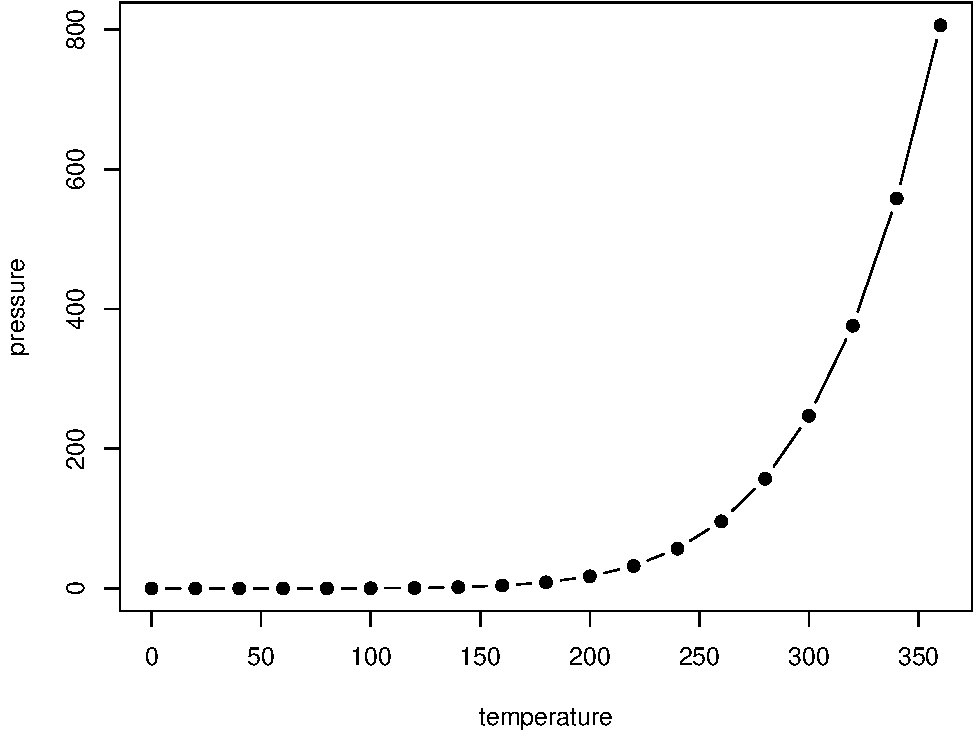
\includegraphics[width=0.8\linewidth]{guia_bolso_R_files/figure-latex/nice-fig-1} 

}

\caption{Here is a nice figure!}\label{fig:nice-fig}
\end{figure}

Don't miss Table \ref{tab:nice-tab}.

\begin{Shaded}
\begin{Highlighting}[]
\NormalTok{knitr}\SpecialCharTok{::}\FunctionTok{kable}\NormalTok{(}
  \FunctionTok{head}\NormalTok{(pressure, }\DecValTok{10}\NormalTok{), }\AttributeTok{caption =} \StringTok{\textquotesingle{}Here is a nice table!\textquotesingle{}}\NormalTok{,}
  \AttributeTok{booktabs =} \ConstantTok{TRUE}
\NormalTok{)}
\end{Highlighting}
\end{Shaded}

\begin{table}

\caption{\label{tab:nice-tab}Here is a nice table!}
\centering
\begin{tabular}[t]{rr}
\toprule
temperature & pressure\\
\midrule
0 & 0.0002\\
20 & 0.0012\\
40 & 0.0060\\
60 & 0.0300\\
80 & 0.0900\\
\addlinespace
100 & 0.2700\\
120 & 0.7500\\
140 & 1.8500\\
160 & 4.2000\\
180 & 8.8000\\
\bottomrule
\end{tabular}
\end{table}

\hypertarget{parts}{%
\chapter{Parts}\label{parts}}

You can add parts to organize one or more book chapters together. Parts can be inserted at the top of an .Rmd file, before the first-level chapter heading in that same file.

Add a numbered part: \texttt{\#\ (PART)\ Act\ one\ \{-\}} (followed by \texttt{\#\ A\ chapter})

Add an unnumbered part: \texttt{\#\ (PART\textbackslash{}*)\ Act\ one\ \{-\}} (followed by \texttt{\#\ A\ chapter})

Add an appendix as a special kind of un-numbered part: \texttt{\#\ (APPENDIX)\ Other\ stuff\ \{-\}} (followed by \texttt{\#\ A\ chapter}). Chapters in an appendix are prepended with letters instead of numbers.

\hypertarget{footnotes-and-citations}{%
\chapter{Footnotes and citations}\label{footnotes-and-citations}}

\hypertarget{footnotes}{%
\section{Footnotes}\label{footnotes}}

Footnotes are put inside the square brackets after a caret \texttt{\^{}{[}{]}}. Like this one \footnote{This is a footnote.}.

\hypertarget{citations}{%
\section{Citations}\label{citations}}

Reference items in your bibliography file(s) using \texttt{@key}.

For example, we are using the \textbf{bookdown} package \citep{R-bookdown} (check out the last code chunk in index.Rmd to see how this citation key was added) in this sample book, which was built on top of R Markdown and \textbf{knitr} \citep{xie2015} (this citation was added manually in an external file book.bib).
Note that the \texttt{.bib} files need to be listed in the index.Rmd with the YAML \texttt{bibliography} key.

The RStudio Visual Markdown Editor can also make it easier to insert citations: \url{https://rstudio.github.io/visual-markdown-editing/\#/citations}

\hypertarget{blocks}{%
\chapter{Blocks}\label{blocks}}

\hypertarget{equations}{%
\section{Equations}\label{equations}}

Here is an equation.

\begin{equation} 
  f\left(k\right) = \binom{n}{k} p^k\left(1-p\right)^{n-k}
  \label{eq:binom}
\end{equation}

You may refer to using \texttt{\textbackslash{}@ref(eq:binom)}, like see Equation \eqref{eq:binom}.

\hypertarget{theorems-and-proofs}{%
\section{Theorems and proofs}\label{theorems-and-proofs}}

Labeled theorems can be referenced in text using \texttt{\textbackslash{}@ref(thm:tri)}, for example, check out this smart theorem \ref{thm:tri}.

\begin{theorem}
\protect\hypertarget{thm:tri}{}\label{thm:tri}For a right triangle, if \(c\) denotes the \emph{length} of the hypotenuse
and \(a\) and \(b\) denote the lengths of the \textbf{other} two sides, we have
\[a^2 + b^2 = c^2\]
\end{theorem}

Read more here \url{https://bookdown.org/yihui/bookdown/markdown-extensions-by-bookdown.html}.

\hypertarget{callout-blocks}{%
\section{Callout blocks}\label{callout-blocks}}

The R Markdown Cookbook provides more help on how to use custom blocks to design your own callouts: \url{https://bookdown.org/yihui/rmarkdown-cookbook/custom-blocks.html}

\hypertarget{sharing-your-book}{%
\chapter{Sharing your book}\label{sharing-your-book}}

\hypertarget{publishing}{%
\section{Publishing}\label{publishing}}

HTML books can be published online, see: \url{https://bookdown.org/yihui/bookdown/publishing.html}

\hypertarget{pages}{%
\section{404 pages}\label{pages}}

By default, users will be directed to a 404 page if they try to access a webpage that cannot be found. If you'd like to customize your 404 page instead of using the default, you may add either a \texttt{\_404.Rmd} or \texttt{\_404.md} file to your project root and use code and/or Markdown syntax.

\hypertarget{metadata-for-sharing}{%
\section{Metadata for sharing}\label{metadata-for-sharing}}

Bookdown HTML books will provide HTML metadata for social sharing on platforms like Twitter, Facebook, and LinkedIn, using information you provide in the \texttt{index.Rmd} YAML. To setup, set the \texttt{url} for your book and the path to your \texttt{cover-image} file. Your book's \texttt{title} and \texttt{description} are also used.

This \texttt{gitbook} uses the same social sharing data across all chapters in your book- all links shared will look the same.

Specify your book's source repository on GitHub using the \texttt{edit} key under the configuration options in the \texttt{\_output.yml} file, which allows users to suggest an edit by linking to a chapter's source file.

Read more about the features of this output format here:

\url{https://pkgs.rstudio.com/bookdown/reference/gitbook.html}

Or use:

\begin{Shaded}
\begin{Highlighting}[]
\NormalTok{?bookdown}\SpecialCharTok{::}\NormalTok{gitbook}
\end{Highlighting}
\end{Shaded}


  \bibliography{book.bib,packages.bib}

\end{document}
